\subsection{Explanation of graph-search based energy management algorithm}
The graph search based energy management solution tested in the paper is designed to be implemented at the point of common coupling (PCC) of a microgrid containing DG and ES. The energy storage management (ESM) solution is in charge of controlling the battery connected to the grid with the objective of getting the most cost optimum use of the available resources. The objective of the ESM is to optimize the use cost of energy storage under changing energy prices taking advantage of load and DG generation forecasting. The inputs of the system are the real-time price (RTP) prediction, load prediction, and the DG output prediction, which in this case is a photovoltaic (PV) plant output. It will also consider the current state of the load, current PV generation, and the state of charge of the ES. The output of the ESM is the optimum battery charge and discharge control references based on the current and forecasted data.

% \begin{figure}[!htbp]
% \centering
% 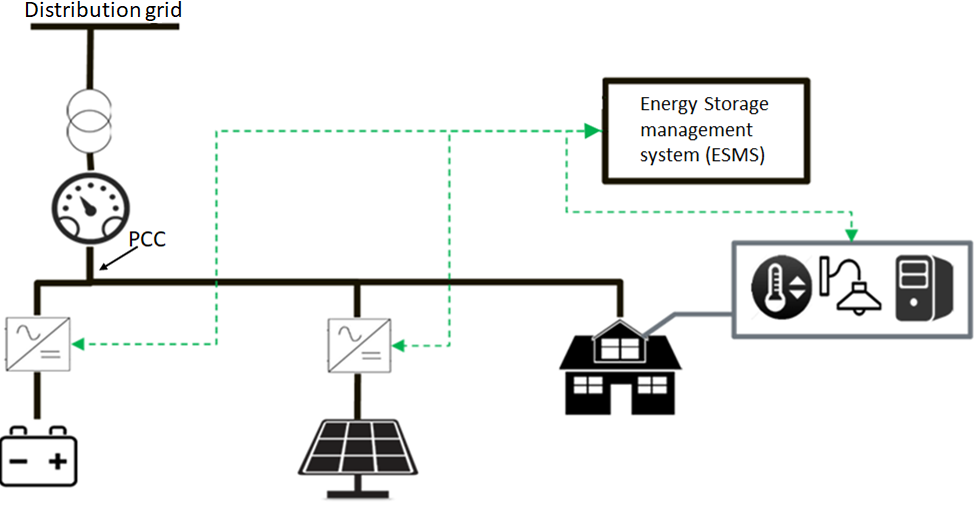
\includegraphics[width=\linewidth]{figs/System_architecture.png}
% \caption{Example test system architecture}
% \label{fig:system_arch}
% \vspace{-3mm}
% \end{figure}

%  Fig. \ref{fig:F1_CA} shows the top-level architecture of the ESMS. As seen in the figure, the inputs of the system are the real-time price (RTP) prediction, load prediction, and the DG prediction, which in this case is a photovoltaic (PV) plant. It will also consider the current state of the load, PV generation, and ES. The output of the ESMS is the optimum battery charge and discharge control references based on the current and forecasted data.

% \begin{figure}[!ht]
%     \centering
%     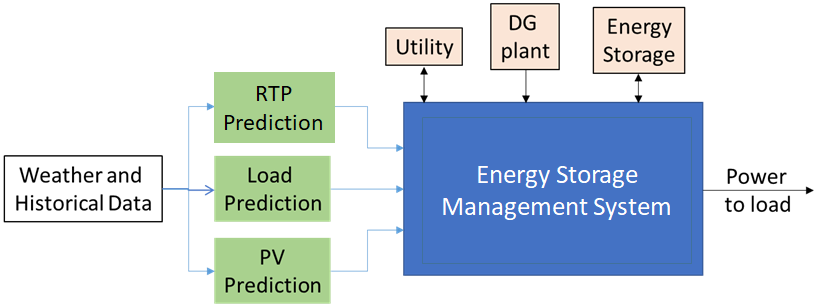
\includegraphics[width = 0.8\linewidth]{figs/EMS_FIG.png}
%     \caption{Controller top level architecture}
%     \label{fig:F1_CA}
% \end{figure}

In order to find the optimum cost solution based on the current status of the system and future forecasts, the optimization problem is formulated using a graph search problem approach. To represent the solution space of the problem as a graph, the state of charge (SOC) of the ES, and both the prediction horizon and the control horizon are discretized. Fig. \ref{fig:F1_Dis} demonstrates an example of the discretized solution space.

\begin{figure}[!ht]
    \centering
    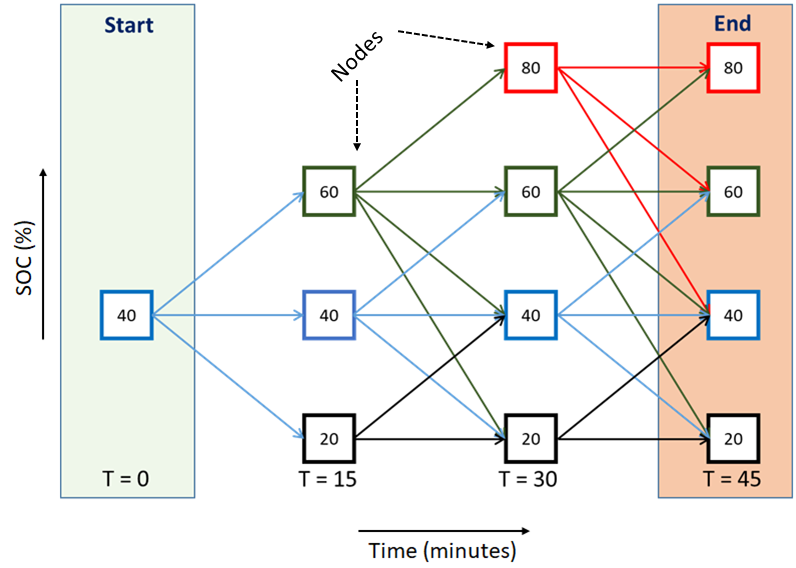
\includegraphics[width = \linewidth]{figs/F1_1_Dis.png}
    \caption{Discretizing solution space of ES as a graph.}
    \label{fig:F1_Dis}
\end{figure}

The horizontal axis of the figure represents time, and the vertical axis represents discrete steps in the state of charge (SOC) of the energy storage. In this simple example scenario, it is assumed that the algorithm recalculates the solution every 15 minutes (control horizon) based on available data. The SOC of the energy storage system (ESS) is discretized in steps of 20\%, and the SOC is limited between 80\% and 20\%. It is also assumed that the ESS can discharge a maximum of 40\% of its maximum SOC and charge a maximum of 20\% of its SOC in a 15 minute time-step. These values are chosen arbitrarily in this simple example scenario to explain the problem. Taking these features into consideration, a directed graph is constructed looking ahead three time-steps into the future. The square boxes represent nodes on the graph. The numbers inside the boxes represent the SOC of the ESS at that node. The arrows from the boxes represent all the possible states the ESS can be in the next time-step according to the constraints of the system. The arrows are treated as edges of the graph. In this case, the edges are unidirectional. The goal is to find the most cost-efficient path to reach T = 45 minutes. Although in this example, the algorithm considers T = 45 as the final stage, in actual application the final stage will be determined based on the actual use case.

The graph search algorithm used to search through the constructed graph is the A* search algorithm. A* is a computer algorithm which is widely used to solve graph search problems. It determines the most efficient path between multiple nodes in a graph. A* is an informed search algorithm. This means, it searches between all the possible paths to the goal and finds the path incurring the least cost. To do this, it considers the paths which appear to have the least cost to get to the goal first. Starting from a specific node, it explores the graph step by step depending on the cost of going from one node to the next. The algorithm selects the node to explore based on a combination of the actual cost to get to the node and a heuristic cost that estimates the cost from the current node to the goal. The process to calculate heuristic cost is problem-specific. For the algorithm to work correctly, the heuristic cost has to be less than or equal to the actual cost of getting to the goal node. In other words, the heuristic cost function should never overestimate the cost of reaching the goal. The algorithm works by calculating the combined actual and heuristic cost for all the neighboring nodes of the starting node and puts them into a priority queue called the \textit{open list}. Then, it selects the node with the least cost and expands that node to get the cost of its neighbors. The expanded node is taken out of the priority queue and put in another list called the \textit{closed list}. The algorithm continues to expand the \textit{open list} always selecting the node with the least cost and adding it to the \textit{closed list}. The algorithm terminates when the goal node is inside the \textit{open list}, and it has the minimum cost in the \textit{open list}. Finally, the algorithm retraces its path through the \textit{closed list} to find the optimum route from start to goal. The following are the main steps of the A* search algorithm.
\begin{enumerate}
% \item \textbf{Set goal node:} Set the goal node as the first component of the predefined list of end nodes. 
%2
\item \textbf{Create the open list from start node:} Expand the start node and create an open list with all the child nodes of the start node. The open list sorts its members in a priority queue based on the cost. The start node is added to the closed list.
%3
\item \textbf{Select and expand the best node from open list:} The node with the lowest cost is selected from the nodes within the open list. The selected node is expanded, and the children of the selected node are added to the open list. The expanded node is then added to the closed list.
%4
\item \textbf{Repeat 3 until goal or stopping criteria is reached}
%5
\item \textbf{Construct shortest path to goal node}: After reaching the goal the shortest path to the goal is constructed from the closed list by retracing the parent nodes from the goal to the start node.
\end{enumerate}

By defining the solution space with a combination of nodes and edges, the optimization problem can be formulated as a graph search problem. At the inception, the starting node is determined by the current status of the system. Then, the following nodes and edges are generated using the forecasted data available. A discrete set of endpoints are set as the goals of the search. The A* algorithm runs for all the goal nodes and the node with the lowest path cost is selected as the best end node. The shortest graph search path to that node is selected as the optimum path.

The EMS recalculates the optimum path using the search algorithm at every time-step based on updated information. The system status is assumed to be constant between time-steps. The cost of going from a parent node to a child node is calculated by combining the real cost of getting to that child node and the heuristic cost of getting to the goal from that child node. The real cost of going from a parent node $p$ at time $T=t$ to a child node $c$ at time $T=t+\Delta T$ is denoted as $C_{actual}(pc)$. It is calculated according to (\ref{eq:C_actual}).
\vspace{-1mm}
\begin{equation}
\label{eq:C_actual}
    C_{actual}(pc) =  C_{ESS}(pc)+C_{GRID}(t)+C_{best}(p)
\end{equation}
\vspace{-1mm}
Here, $\Delta T$ represents the time between two time-steps. $C_{actual}(pc)$ represents the total cost of going to the child node $c$ from parent node $p$. $C_{ESS}(pc)$ represent cost of energy storage to go from parent node $p$ to child node $c$. $C_{GRID}(t)$ is the cost of using the grid between time $T=t$ and time $T=t+\Delta T$. $C_{best}(p)$ represent the best or least cost to get to the parent node $p$ from the start node. $C_{ESS}(pc)$ is calculated according to (\ref{eq:C_ESS}).
\vspace{-1mm}
\begin{equation}
\label{eq:C_ESS}
C_{ESS}(pc) = |(SOC_p - SOC_c)|*ESS_{CAP}*R_{ESS}
\end{equation}
\vspace{-1mm}
Here, $SOC_p$ and $SOC_c$ represent the state of charge at parent and child node. $ESS_{CAP}$ represent the total energy capacity of the energy storage. And $R_{ESS}$ is the $\$/kWh$ cost of using the energy storage. $C_{GRID}(t)$ is calculated according to (\ref{eq:C_GRID}).
\vspace{-1mm}
\begin{equation}
\label{eq:C_GRID}
C_{GRID}(t) = 
\begin{cases}
   E_{GRID}(t)*RTP(t),& \text{if } E_{GRID}(t)\geq 0\\
    E_{GRID}(t)*SP(t),& \text{if }  E_{GRID}(t) < 0
\end{cases}
\end{equation}
\vspace{-1mm}
Here, $E_{GRID}(t)$ is the energy drawn from the grid between time $T=t$ and time $T=t+\Delta T$. $RTP(t)$ is the real-time price between $t$ and $t+\Delta T$. $SP(t)$ is the price the utility is willing to pay to the consumer for selling power between $t$ and $t+\Delta T$. The heuristic cost is calculated by assuming that whichever source has the smallest cost during a time-step will supply the total energy demand of that particular time-step. The heuristic cost of a node at time $T = t$ is calculated according to (\ref{eq:C_H}).

\vspace{-1mm}
\begin{equation}
\label{eq:C_H}
C_H(t) = \sum_{n=t}^{end} D(n)*R_{best}(n)
\end{equation}
\vspace{-1mm}
Here, $C_H(t)$ represents the heuristic cost at time $t$. $D(n)$ is the demand between time $T = n$ and time $T = n+\Delta T$. $R_{best}(n)$ is the source with the smaller cost which is calculated according to (\ref{eq:R_best}).
\vspace{-1mm}
\begin{equation}
\label{eq:R_best}
R_{best}(t) = 
\begin{cases}
    R_{ESS},& \text{if } RTP(t)\geq R_{ESS}\\
    RTP(t),              & \text{otherwise}
\end{cases}
\end{equation}
\vspace{-1mm}
After calculating the actual cost  $C_{actual}(pc)$ and heuristic cost $C_H(t)$, the total cost is finally calculated by adding  $C_{actual}(pc)$ and $C_H(t)$. 





% \subsection{Generic explanation of Voltage Control Algorithm}

% \subsection{Generic explanation of EM - GA,PSO}